\chapter{E1-f}
\label{cha:E1f}

The E1-f run at Jefferson Lab operated from April through June of 2003 and contains approximately 2 billion triggers.
The run used a 5.498 GeV electron beam with a 75.1$\pm$0.2\% polarization.
The target was unpolarized liquid hydrogen.
It was determined that running the torus magnet at 60\% of its maximum value (which is given in~\cite{Mecking03} as $\int B \cdot dl \approx 1.7\ \text{T} \cdot m$) would improve acceptance.
Both charged pion channels - $\pi^+$ and $\pi^-$ - were binned and studied in a fully differential way over a broad kinematic range ($0.1 < x < 0.6$, $1.0 < Q^2 < 4.7\ \text{GeV}^2$, $0.0 < z < 0.9$, $0.0 < P_{h\perp}^2 < 1.0\ \text{GeV}^2$, and $-180^\circ < \phi_h < 180^\circ$) within SIDIS kinematic cuts ($W > 2.05$ GeV, $y < 0.85$, and $Q^2 > 1.0\ \text{GeV}^2$) (see figure~\ref{fig:binningScheme}).

The binning scheme, shown by gray lines in figure~\ref{fig:binningScheme}, is defined in the following way:
\begin{itemize}
\item $x$: 5 equally spaced bins from 0.1 to 0.6.
\item $Q^2$: 2 bins in $Q^2$ for each $x$ bin except for the largest $x$ bin which has only 1 $Q^2$ bin. The upper and lower bounds are defined by the cuts on $W$, $y$, and $Q^2$ mention above. The 4 $Q^2$ values defining the dividing lines between the high and low $Q^2$ bins for the first 4 $x$ bins are 1.3, 1.7, 2.2, and 2.9 $GeV^2$.
\item $z$: 18 equally spaced bins from 0.0 to 0.8.
\item $P_{h\perp}^2$: 20 equally spaced bins from 0.0 to 1.0 $GeV^2$.
\end{itemize}

The resolution for each kinematic variable is a function of the kinematics, the resolution range for each variable is
\begin{itemize}
\item $x$: 0.001 - 0.009
\item $Q^2$: 0.006 - 0.15 $GeV^2$
\item $z$ ($\pi^+$): 0.0008 - 0.008
\item $P_{h\perp}^2$ ($\pi^+$): 0.0008 - 0.038 $GeV^2$
\item $\phi_h$ ($\pi^+$):  0.7 - 3.4 degrees
\item $z$ ($\pi^-$): 0.001 - 0.014
\item $P_{h\perp}^2$ ($\pi^-$): 0.0014 - 0.147 $GeV^2$
\item $\phi_h$ ($\pi^-$):  0.86 - 2.1 degrees.
\end{itemize}
where the above numbers are sigmas from gaussian fits of the generated - reconstructed distributions from the Monte Carlo simulations.
%
\begin{figure}[htp]
\centering
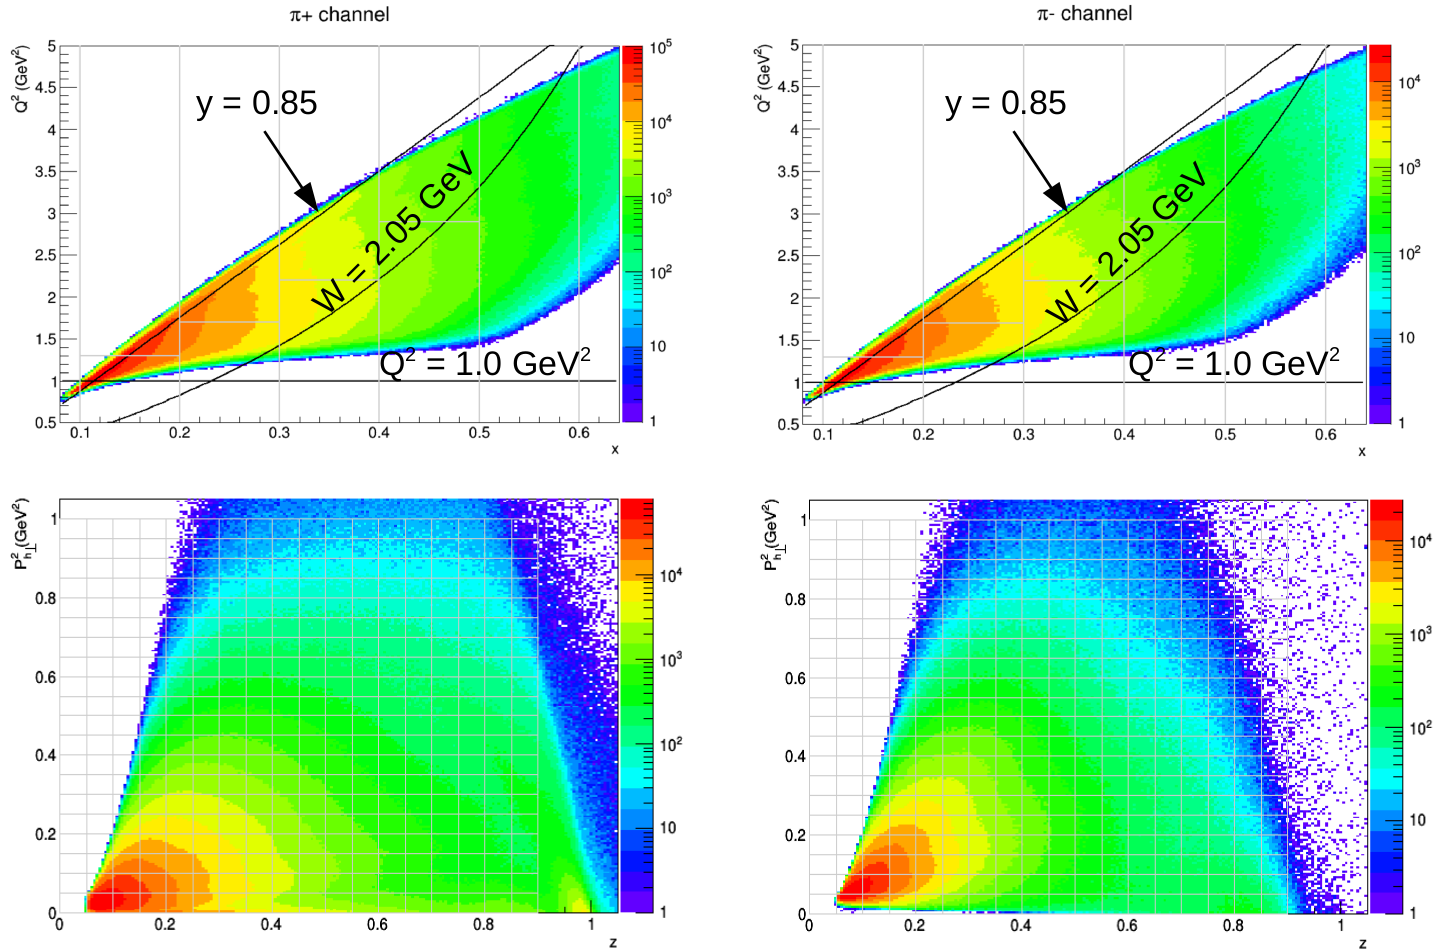
\includegraphics[width=4.5in]{figures/binningScheme.png}
\caption{The $x$-$Q^2$ (top) and $z$-$P_{h\perp}^2$ (bottom) kinematic coverage and binning scheme (gray lines) for $\pi^+$ (left) and $\pi^-$ (right) for the E1-f data set.}
\label{fig:binningScheme}
\end{figure}


